\documentclass[12pt]{article}
\usepackage[utf8]{inputenc}
\usepackage[T1]{fontenc}
\usepackage{lmodern}
\usepackage{graphicx}
\usepackage{subcaption}
\usepackage[svgnames]{xcolor}
\usepackage[a4paper,bindingoffset=0.2in,%
            left=0.5in,right=0.5in,top=0.5in,bottom=1in,%
            footskip=.25in]{geometry}
\pagenumbering{gobble}
\usepackage[colorlinks=true, linkcolor=Black, urlcolor=Blue]{hyperref}

\begin{document}
\title{Sprawozdanie z zajęć z prototypowania}
\author{Sebastian Michoń 136770, Mateusz Wankowski 136823,\\ Piotr Król 136745, Maciej Leszczyk 136759}
\date{\vspace{-3ex}}
\maketitle

\section{Idee, koncepcje, motywacje}
Ideą naszego prototypu było stworzenie aplikacji wspomagania systemu kolejkowego, podobnej do politechnicznego Zintegrowanego Centrum Obsługi. Uznaliśmy, że aplikacja politechniczna powinna pomagać zaoszczędzić czas studentom. Skłoniło nas to do stworzenia nowej, lepszej wersji tego systemu z dodatkiem kilku ciekawych funkcji. Nasza aplikacja ma charakter mobilny, co umożliwia korzystanie z niej poza politechniką oraz zaoszczędza czas który traciliśmy czekając w kolejce.

\section{I etap prototypowania}
\subsection {Indywidualne pomysły}
\begin {enumerate}
	\item Pierwsza koncepcja indywidualna Piotra to możliwość stwierdzenia, przy pobraniu biletu, czy dana osoba zgadza się na przesuwanie jej w kolejce na wcześniejszy termin. Uznaliśmy, że jeśli osoba ma termin wizyty o kilka godzin późniejszy niż termin pobrania biletu, może chcieć na przykład zjeść obiad w trakcie czasu oczekiwania - natomiast jeśli i tak czeka w poczekalni, może się zgodzić na przesuwanie jej na jak najwcześniejszy termin, jeśli jakaś wizyta potrwa krócej niż oczekiwano albo ktoś zrezygnuje z wizyty.
	
	\item Mateusz zauważył, że czekając w kolejce często nie mamy niczego ciekawego do robienia i dobrze by było umilić ten czas studentom, dzięki możliwości komunikowania się z innymi osobami w kolejce. Do tego celu stworzyliśmy substytut messengera, który umożliwia dołączenie do czatu grupowego, oraz wysyłania wiadomości prywatnych. Dla osób niezainteresowanych czatem przewidzieliśmy możliwość wyłączenia komunikacji.
	
	\item Pomysł Macieja to umożliwienie przeglądania osób znajdujących się razem z nami w kolejce. Po zalogowaniu się i dołączeniu do poczekalni użytkownik widzi swoje informacje personalne wraz ze zdjęciem, numerkiem w kolejce oraz szacowanym czasem oczekiwania. Oprócz tego interfejs wyposażony jest w guziki next i previous dzięki którym użytkownik może dostrzec analogiczne informacje o innych uczestnikach z kolejki.
	
	\item Sebastian spostrzegł, że dobrze by było, gdyby osoba zalogowana do systemu miała możliwość obejrzenia swojej historii wizyt w dziekanacie - żeby przypomnieć sobie, z kim ostatnio prowadziła konwersację na przykład po to, żeby później móc dostarczyć mailem zaległą informację, której nie była w stanie podać w trakcie wizyty.

\end {enumerate}

\subsection {Co wspólne, co różne}
Wspólną cechą wszystkich projektów były dwie nowe funkcjonalności - ekran logowania do systemu i mechanizm szacowania czasu pozostałego do wizyty. Poza wyżej wymienionymi funkcjonalnościami, wszystkie pomysły były inne od siebie. 

\subsection{Co okazało się dobrym pomysłem, co nie}
\begin {enumerate}
	\item Chat okazał się badzo dobrym pomysłem. Jednoznacznie uznaliśmy, że bardzo dużo studentów chętnie kożystałoby z możliwości komunikowania się z innymi osobami.
	
	\item Możliwość stwierdzenia, czy osoba woli być przesuwana w kolejce także jest opcją, która jest z naszej perspektywy bardzo zasadna - przy długim czasie oczekiwania danie użytkownikowi możliwości przyjścia o konkretnej godzinie pozwala mu spożytkować swój czas na inne aktywności niż stanie w kolejce.
	
	\item Historia poprzednich wizyt okazała się przeciętnym pomysłem. Niektórzy uważają, że zdecydowana większość użytkowników nie będzie miała potrzeby z niej skorzystać. Taka funkcjonalność może natomiast stanowić pomoc dla niektórych osób i w szybki i wygodny sposób przekazywać potrzebne informacje.
	
\end {enumerate}

\section {Wnioski z II etapu projektowania aplikacji}
\subsection {Które pomysły zostały zrealizowane, które nie?}

Wszystkie indywidualne pomysły zostały zaimplementowane w naszej aplikacji, jednak część z nich w inny sposób niż wyobrażał to sobie autor - w pełni zrealizowaline zostały koncepcje historii i zgody na przesuwanie w kolejce, z kolei chat został połączony z możliwością przeglądania użytkowników w kolejce.

\subsection{Które pomysły okazały się trafione, które nie według osób spoza grupy?}
\begin{enumerate}
	\item Trafionym pomysłem okazał się chat razem z możliwością przeglądania innych osób znajdujących się w kolejce - ludzie spoza grupy byli bardzo skorzy do korzystania z tej funkcjonalności aplikacji, niekiedy nawet bardziej niż z jej głównej funcjonalności.
	\item Prosta funkcjonalność zgody na przesuwanie w kolejce zgodnie z oczekiwaniami nie wzbudzała wielkiego zainteresowania, natomiast różne osoby wybierały albo nie wybierały tą opcję - a co za tym idzie, była zauważana i spełniała swoje zadanie.
	\item Historia wzbudzała kontrowersje - jedni twierdzili, że jest absolutnie zbędna, inni, że może być bardzo pomocna w dostarczaniu potrzebnych informacji.
\end{enumerate}


\clearpage


\begin{figure}[h!]
	\section {Aplikacja w akcji}
	\subsection{Wygląd całej aplikacji}
	\centering
	\begin{subfigure}[b]{1\linewidth}
		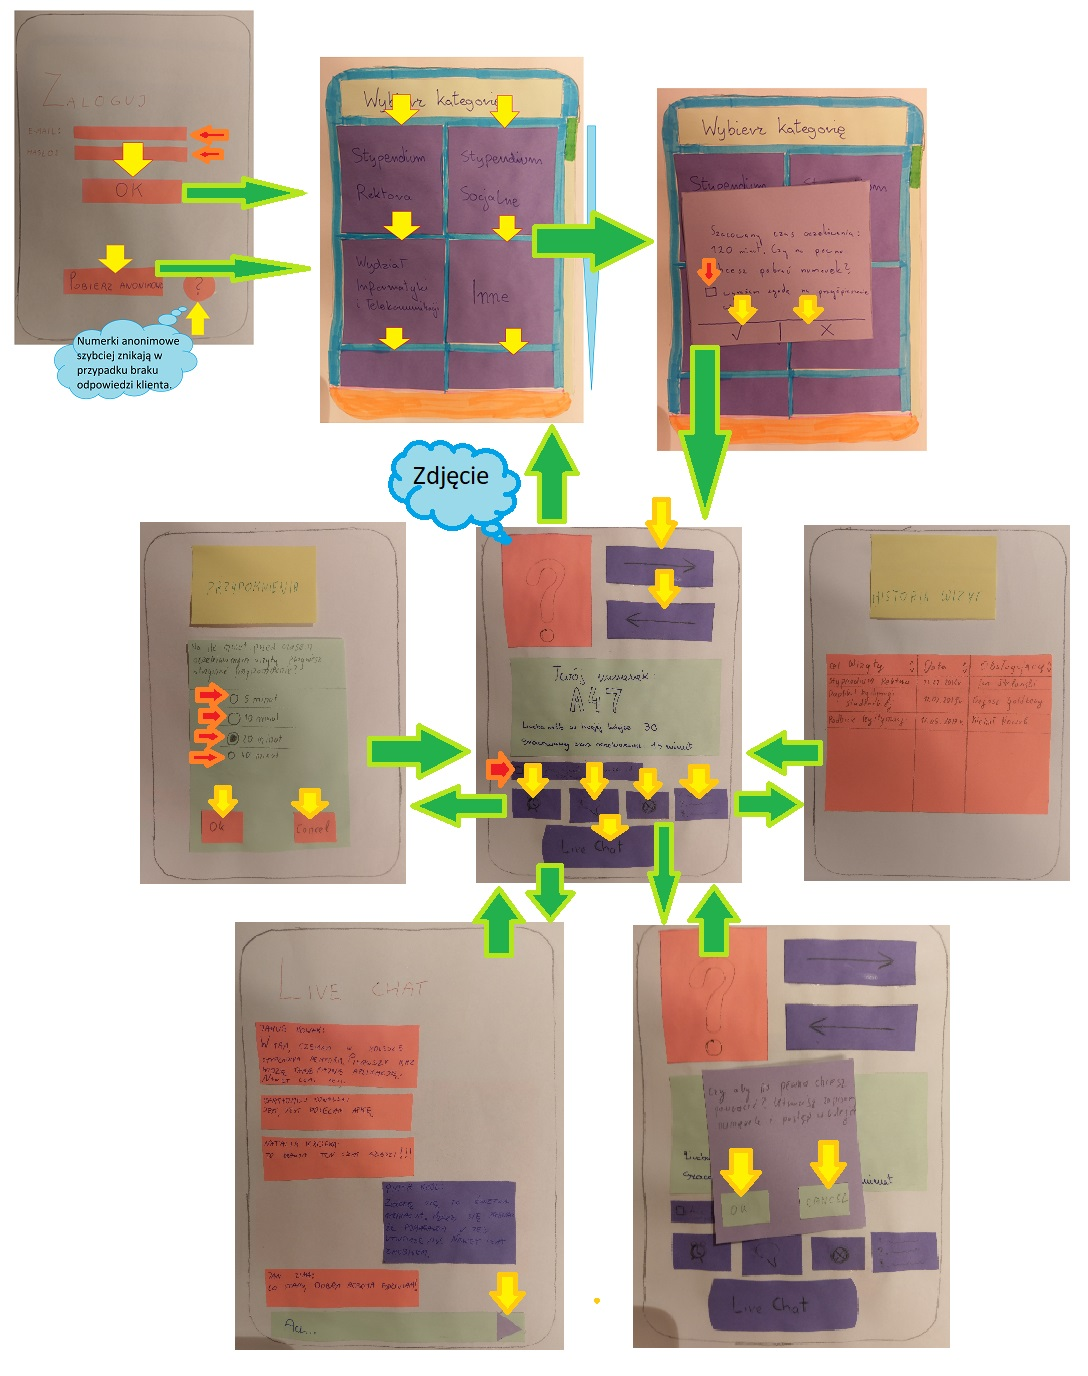
\includegraphics[width=\linewidth]{zdj/mozaika.jpg}
		\caption{\underline{Podpis}}
	\end{subfigure}
	\label{fig:nuty}
	\caption{Nawigacja}
\end{figure}

\clearpage
\subsection{Działanie aplikacji:}
\begin {enumerate}
	\item Pierwszym ekranem, na który natrafi użytkownik korzystający z aplikacji jest ekran "zaloguj". Są na nim 2 pola tekstowe na email i hasło do politechnicznego ekonta, a także przyciski: "zaloguj", "pobierz anonimowo" i "?". Przycisk "?" podaje informację o szybszym znikaniu numerków anonimowych. Jeśli użytkownik poda złe hasło/login, po kliknięciu przycisku "OK" wyświetli się czerwony komunikat pod przyciskiem "OK": "Niepoprawne dane logowania". Oczywiście "Pobierz anonimowo" pozwala przejść do następnego okna bez logowania.
	
	\item Drugi ekran to ekran wyboru kategorii. Są tam takie opcje, jak: "Stypendium rektora", "Leigtymacja studencka", "Stypendium socjalne", a także kategoria specjalna, nie powodująca pobrania numerka: "Historia".
	
	\item Po wybraniu kategorii różnej od historii pokazuje się komunikat: "Szacowany czas oczekiwania: ${x}$ minut. Czy na pewno chcesz pobrać numerek? Niżej jest checkbox "Wyrażam zgodę na przyspieszenie wizyty". Zaznaczenie checkboxa powoduje, że czas oczekiwania może się zmniejszyć. Użytkownik może kliknąć "v"(wziąć numerek) lub "x" (nie wziąć numerka).
	
	\item Po wzięciu numerka ukazuje się ekran główny. Znajdują się na nim zdjęcie użytkownika, strzałki w lewo i prawo, numerek w kolejce, czas oczekiwania oraz liczba osób przed użytkownikiem. Strzałki umożliwiają przeglądanie profilów innych użytkowników znajdujących się w kolejce. Na dole ekranu znajdują się cztery przyciski - przycisk ze znakiem budzika prowadzący do ekranu przypomnień, przycisk ze znakiem chmurki powodujący przejście do ekranu chatu prywatnego, przycisk ze znakiem listy numerowanej prowadzący do ekranu historii, przycisk z napisem "Live Chat" prowadzący do czatu grupowego, przycisk ze znakiem 'x' w kółku, tak samo jak kliknięcie przycisku powrotu w telefonie, powodujący wyświetlenie komunikatu z ostrzeżeniem "Czy na pewno chcesz powrócić? Stracisz numerek i postęp w kolejce".
	
	\item Ekran historii przedstawia tabelę z celami wizyt, ich datą oraz nazwiskiem osoby, z którą rozmawialiśmy. Dane można sortować dla wygody przyciskami "\^{}" i "v" przy nagłówku kolumny. Kliknięcie powrotu na telefonie prowadzi do okna głównego albo okna kategorii, zależnie od poprzedniego okna.
	
	\item Ekran przypomnień pozwala na ustawienie przypomnienia na $x$ minut przed wizytą, gdzie $x\in\{5, 10, 20, 40\}$. Przycisk "OK" ustawia przypomnienie, przycisk "Cancel" usuwa ustawione wcześniej przypomnienie. Powrót na telefonie po prostu wraca do poprzedniego ekranu (ekran główny)
	
	\item Ekran chatu występuje w aplikacji w dwuch formach: konwersacji grupowej oraz prywatnej. Informacja o formie chatu znajduje się na górze ekranu. Ekran ten pozwala na wysyłanie wiadomości poprzez wprowadzenie ich w prostokątne pole na dole ekranu oraz naciśnięcie przycisku ze znakiem strzałki w prawo. Wiadomości innych użytkowników wraz z ich imionami i nazwiskami wyświetlane są po lewej stronie w pomarańczowych chmurkach, natomiast informacje wysłane przez zalogowanego użytkownika po stronie prawej w niebieskich chmurkach
	
\end{enumerate}


\clearpage
\subsection{Przykaładowe scenariusze}
(kursywą oznaczone są zalety aplikacji pokazane w scenariuszu i elementy ewaluacji heurystcznej)
\begin {enumerate}
	\item Użytkownik A postanawia złożyć wniosek o stypendium rektora. Loguje się do systemu, wybierając kategorię "Stypendium Rektora". Dostaje informację - szacowany czas oczekiwania to 150 minut. Uznaje, że lepiej spożytkuje ten czas idąc do restauracji i spożywając tam obiad niż czekając w poczekalni. Z tego powodu nie zaznacza checkboxa "Wyrażam zgodę na przyspieszanie wizyty", klikając od razu na przycisk v. Po naciśnięciu przycisku wyświetlany jest ekran profilu użytkownika. Znajduje się na nim jego numerek oraz czas oczekiwania 150 minut. Użytkownik uznaje, że dobrze byłoby ustawić sobie przypomnienie, aby nie zapomnieć o wizycie. W tym celu wybiera znaczek budzika, następnie dotyka checkboxa przy napisie "20 minut" i klika OK, przechodząc tym samym do ekranu głównego. Użytkownik po otrzymaniu przypomnienia ok. 130 minut później przybywa do dziekanatu, rozwiązuje swój problem i zamyka aplikację.
	
	\textit{Aplikacja nie komunikuje zbędnych informacji - użytkownik nie musi analizować rozległych okien dialogowych, jedynie bardzo mały zbiór informacji niezbędnych do uzyskania oczekiwanego przez niego efektu, a co za tym idzie, jeśli jakiś komunikat aplikacji jest użyteczny to prawie na pewno zostanie spostrzeżony przez użytkownika.}\\
	
	
	\item Użytkownik B postanawia wyrobić duplikat legitymacji studenckiej. Loguje się zatem do systemu wybierając opcję "Legitymacja Studencka". Otzymuje informację o tym, że szacowany czas oczekiwania to 70 minut. Uznaje, że spędzi ten czas w poczekalni, dlatego zgadza się na przesuwanie wizyty na wcześniejszy termin. Użytkownik następnie klika przypadkowo na znak powrotu w telefonie, widząc chwilę później komunikat "Czy na pewno chcesz powrócić? stracisz numerek i postęp w kolejce" klika przycisk cancel, ponieważ nie taka jest jego wola. Następnie wybiera opcję "Live Chat", aby zająć czymś czas i rozpoczyna konwersację z innymi użytkownikami tej aplikacji. Gdy nadchodzi czas na obsługę jego numerka wchodzi do dziekanatu, rozwiązuje swój problem i zamyka aplikację.
	
	\textit{Komunikaty ostrzegawcze są przedstawione w prostym języku i jednoznacznie wskazują na konsekwencję danego działania; istnieje wyjście ratunkowe z niechcianej sytuacji.}\\
	
	\item Użytkownik C postanawia skorzystać anonimowo z aplikacji po przeczytaniu informacji "Numerki anonimowe szybciej znikają w przypadku braku odpowiedzi klienta" zauważonej po kliknięciu w przycisk "?". Wybiera opcję "Stypendium socjalne", otrzymuje komunikat "Szacowany czas oczekiwania: 13726 miunt. Czy na pewno chcesz pobrać numerek?". Uznaje, że nie zamierza czekać 229 godzin w kolejce, dlatego klika "x" i zamyka aplikację.
	
	\textit{Unikamy sytuacji w których użytkownik pobiera numerek, a następnie rezygnuje z niego. Istnieje wyjście ratunkowe z niechcianej sytuacji.}\\
	
	
	\item Użytkownik D chce jedynie dosłać przez maila informację dla osoby, która poprzednio go obsługiwała, dlatego po zalogowaniu się wybiera kategorię historia(do użycia której nie potrzebuje numerka). Sprawdza, kto ostatnio go obsługiwał w dziekanacie, aby później wysłać tej osobie maila, następnie zamyka aplikację.\\
	
	\textit{Wymienione sytuacje pokazują funkcjonalność aplikacji. Interfejs użytkownika daje wiedzę o tym, co się dzieje w systemie. Poza ekranem głownym użytkownik zawsze widzi na szczycie aplikacji nazwę ekranu, z którego aktualnie kożysta. Wszystkie opcje są widoczne z poziomu ekranu głównego. Komunikaty są jednoznaczne, nie dają dużej przestrzeni na błędne interpretacje.}

\end{enumerate}

\end{document}
